\usepackage{}%% Template for SDP report, adapted from mlp_cw2_template, 2018. 

%% Based on  LaTeX template for ICML 2017 - example_paper.tex at 
%%  https://2017.icml.cc/Conferences/2017/StyleAuthorInstructions



\documentclass{article}

\usepackage[T1]{fontenc}
\usepackage{amssymb,amsmath}
\usepackage{txfonts}
\usepackage{microtype}
\usepackage{xspace}
\xspaceaddexceptions{\%}
\usepackage{subcaption}
% Lists with less spacing between items
\usepackage{paralist}
\usepackage{tabularx}
\usepackage[normalem]{ulem}
% For figures
\usepackage{graphicx}
\usepackage{subfig} 

% For citations
\usepackage{natbib}

% For algorithms
\usepackage{algorithm}
\usepackage{algorithmic}

% the hyperref package is used to produce hyperlinks in the
% resulting PDF.  If this breaks your system, please commend out the
% following usepackage line and replace \usepackage{mlp2017} with
% \usepackage[nohyperref]{mlp2017} below.
\usepackage{hyperref}
\usepackage{url}
\urlstyle{same}

% Packages hyperref and algorithmic misbehave sometimes.  We can fix
% this with the following command.
\newcommand{\theHalgorithm}{\arabic{algorithm}}


% Set up MLP coursework style (based on ICML style)
\usepackage{mlp2018}
\mlptitlerunning{SDP Demo \demoNumber  Group (\groupNumber)}
\bibliographystyle{icml2017}


\DeclareMathOperator{\softmax}{softmax}
\DeclareMathOperator{\sigmoid}{sigmoid}
\DeclareMathOperator{\sgn}{sgn}
\DeclareMathOperator{\relu}{relu}
\DeclareMathOperator{\lrelu}{lrelu}
\DeclareMathOperator{\elu}{elu}
\DeclareMathOperator{\selu}{selu}
\DeclareMathOperator{\maxout}{maxout}






\usepackage{tikz}
\usepackage[justification=centering]{caption}
\usepackage{gensymb}
\def\checkmark{\tikz\fill[scale=0.4](0,.35) -- (.25,0) -- (1,.7) -- (.25,.15) -- cycle;}

%% You probably do not need to change anything above this comment

%% REPLACE the details in the following commands with your details
\setGroupNumber{4}
\setGroupName{Sprout.ed}
\setProductName{Sprout.ed}
\setDemoNumber{1}
\setLogoFileName{figs/sprouted_logo.png}
\begin{document} 

\makeSDPTitle{Demo}

% Previous MLP Style Title Layout working. 
% \twocolumn[
    % \mlptitle{\productName: SDP Demo \demoNumber}
    % \centerline{Group \groupNumber: \groupName}
% ]

\begin{abstract}
Sprout.ed currently consists of a gantry which can move back and forth along a set of rails, accompanied by a web interface which allows for the sending of commands to the gantry base motors and the display of data from attached sensors. These are the first steps towards a 3 axis planting system designed for office space usage, with a web app allowing for an overview and management of the currently growing plants. 

Mechanically, we were able to construct the gantry and design 3D printed parts which allowed us to join the aluminium struts to the EV3 motorised LEGO bases, these bases went through a few iterations to reduce the strain on the powered wheel. We also set up a Flask web server on the Raspberry Pi which is used as an interface to send commands or display sensor readings at the click of a button, the former required creating a TCP server on the Pi in order to facilitate communication to the EV3.
\end{abstract} 
\vspace{-8mm}

\section{Project plan update} 

\subsection{Milestone 1 goal updates}
\textbf{Goals:}
\begin{enumerate}
    \vspace{-3mm}
    \setlength{\itemsep}{0pt}%
    \setlength{\parskip}{0pt}
    \item (Achieved) Frame of the robot set up with the gantry that can move in one axis. 
    \item (Achieved) Communication from Web Interface to Motors via server on Raspberry Pi.
    \item (Achieved) Sensors are set up to sense soil moisture and temperature.
    \item (Achieved) Web server set up.
    \item (Achieved) Communication between Raspberry Pi and web app established.
    \item (Achieved) Wireframe of the web page.
    
\end{enumerate}

We were organized into three sub-teams when working towards this milestone.

The \textbf{Mechanical team} achieved 100\% of our targets for Milestone 1 The sub-team members drafted together a design for the movable gantry, then decomposed the task to all all members of the team to work simultaneously. Yichao and Rokas built the frame of the robot and Anukrat built a prototype design for the adapter using LEGO\textsuperscript{\textregistered}. Yichao then worked on modelling and 3D printing an adaptor that connects the metal struts and the LEGO\textsuperscript{\textregistered} motorised gantry base, while Rokas worked on optimizing the motor base's efficiency and stability on the rails. Anukrat measured the dimensions of the designed adaptor and the wooden board (base). Anukrat also worked on the overall budget of the hardware team. The sub-team has spent £58.15 and 30 minutes of technician time so far, with more details about the estimated total cost provided in Section \ref{budget_account}.



The \textbf{Electrical team} achieved all of our predefined targets for Milestone 1. To achieve our tasks, we decided to divide the team based on experience and level of collaboration required with other sub-teams. Alan, who had some experience with web development and EV3s, worked closely with the Web Application team to establish communication between the Web App and the Motors. Alan and Balraj used Git for version control and adopted the Pair Programming technique. Meanwhile, Shreyas, Terry, and Serena worked on first establishing a connection between the Raspberry Pi and the Moisture and Temperature Sensors, and then outputting this information to the web app. For the latter stage, they worked closely with Sonia and Balraj from the Web Application Team.


The \textbf{Web Application team} achieved all goals set for Milestone 1 and additionally went beyond making a wireframe design of the application, to making an interactive prototype. This was more useful as it allowed us to show the app to other people in order to gather valuable feedback on user experience. We had initial problems when setting up the web server, relating to WiFi connection on the Raspberry Pi, which many team members worked on resolving. Sonia then set up a basic web application hosted on the Raspberry Pi, meeting the milestone of setting up a web server. After discussing the essential functionality required as a whole sub-team (Sonia, Balraj, Dima) and making initial basic wireframes using paper then Google Slides, we split off on different tasks to make efficient use of time. Dima and Sonia worked together to build the prototype using the collaborative interface design tool, Figma. Meanwhile, Balraj worked with Alan from the Electrical team to set up the communication between the web app and the motors. 




\subsection{Milestone 2 goal modifications}
Having reached Demo 1 and achieved our Milestone 1 goals, we have now considered the next steps and made the following modifications to the goals for Milestone 2. 
\textit{(The \textbf{Mechanical team} has no goal modifications.)}

\textbf{Electrical team}: The sensor group succeeded in displaying the readings on the Web interface, thus completing one part of our Milestone 2. This milestone will be replaced with the following:
\begin{itemize}
    \vspace{-2mm}
    \setlength{\itemsep}{0pt}%
    \setlength{\parskip}{0pt}
    \item Set up a Cartesian Grid system
    \item Trigger movement of head based on low soil moisture levels
\end{itemize}

\textbf{Web Application team}:
We are modifying the Milestone 2 goal of 'Sensor data display' to clarify this goal. In addition, our goal of 'Sending commands to manually move in any of the three axes' depends on the Mechanical team completing their goals for milestone 2, and is more relevant to the Electrical team, so to make more efficient use of time we have removed this goal. Our updated set of goals for Milestone 2 is the following:
\begin{itemize}
    \setlength{\itemsep}{2pt}
    \setlength{\parskip}{0pt}
    \setlength{\topsep}{0pt}
    \item Display updated sensor data at a time interval and graphs of sensor data history
    \item Implement basic UI
    \item Implement data structure to store plant data and allow addition and removal of plants
\end{itemize}



\section{Technical details}



\subsection{Mechanical team}
The first milestone of the mechanical team was building a movable gantry. The gantry consists of two rails and a \(\Pi\)-shaped frame that would move along them, with its legs placed over each rail. 
The gantry had to be stable but also tall enough to not interfere with plants, and the easiest way to achieve this was using pre-cut aluminium struts. This allowed a very fast construction of the prototype with high structural integrity. These parts were mostly chosen for their convenience, as they have notches for fittings and equal length parts were available pre-made. Before discovering these parts, we considered building the gantry out of LEGO, which would have required a lot more effort, resources and time and end up being significantly flimsier, or cutting our own wood parts. This extra time required would have meant the electrical team could not have tested gantry movement properly. Additionally, the weight of the struts allows us to stress test our system early-on and design parts that can withstand higher weight than they would encounter under normal ciscumstances.
\\ \\
Two LEGO bases were constructed to move the gantry along the track. These went through several iterations (shown in Figure \ref{fig:stages}) to find a design that would be stable and minimize friction. For the latter goal, supporting wheels were used. The first two iterations used wheels extending from the sides of the base and lowered from the rail for stability, but after noticing that weight of the gantry bends them, the stabilization was provided by parts which slot into the notches under the rails. Since the addition of wheels, removing the rails completely was briefly considered, but ultimately decided against, since our use-case would not involve a surface appropriate for wheels without the rail bases, and the gear fitted into the rail provides additional stability and precision when moving. \\ Concerns as to whether the motors can move the weight of the gantry were alleviated thanks to an SDP project last year which also utilised a gantry system, although replacing part of the gantry with a lighter one is still considered.
\\ \\
Lastly, the gantry and LEGO bases had to be connected. We used a custom made 3D printed adaptor that snaps onto the LEGO base and slot in the gantry leg on top. This simplifies the structure, takes up less volume (compared to one built with LEGO), and adds stability for future building. The \textit{Ultimaker} PLA filament was chosen to 3D print the adaptor with an infill density of 20 percent to achieve a balance between strength and cost. Due to the importance of this part for the general stability of the system, hardest possible material was considered, but after examining other models printed with the setting mentioned earlier, we discovered that they were more than sufficient (and cheaper). The model of the custom fitting was provided by the technicians and was incorporated into the model of the adaptor. The adaptor had two iterations, since measurements were slightly off in the first iteration. Models from both iterations are being used at the moment, as the first iteration is still functional after some manual adjustments. Initially, a design with four walls was considered, where the gantry would be slotted in. However, we decided that we could save a significant amount of material and provide greater stability by exploiting the notches available on the rods. \\
\label{sec:stages}
\begin{figure}[h!]
    \centering
    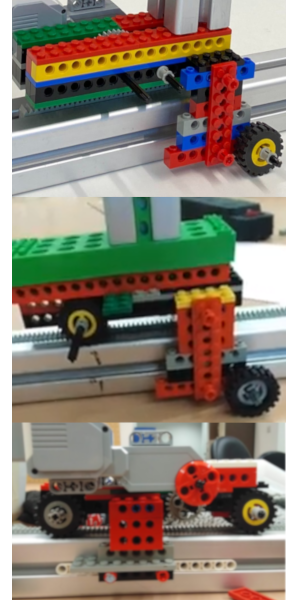
\includegraphics[height=280,keepaspectratio,width=1\linewidth]{figs/stagesofbase.png}
    \caption{From top to bottom: iteration 1 through 3 of the gantry base}
    \label{fig:stages}
\end{figure}

\subsection{Electrical team}

To establish the web server - motor connection the python socket interface and \href{https://github.com/imgeorgiev/tcpcom}{tcpcom} library was used.

On booting, the Raspberry Pi starts a Flask web server and a TCP server which run simultaneously. The EV3, on booting, runs the client code which sets up a permanent connection with the TCP server running on the Pi. On clicking a button on the front end, a command  (eg: “Move Motors”) is sent to the web server (on the Raspberry Pi) which initialises a connection with the TCP server (also running on the Pi). On connecting, it forwards the command to the TCP server and then disconnects itself. On receiving the command, the TCP server sends the message to the EV3 client which then makes a move according to the command.



We decided to have all the "heavy-lifting" (running servers, forwarding messages and decision making) done by the Raspberry Pi while the EV3 listens to more low-level commands like “Move Motors Forward” because we found the EV3 to be much slower when compared to the Raspberry Pi.


The EV3 is used to run and power the motors instead of the Raspberry Pi because there is a risk of overheating the Pi since it is not designed to control the kind of amperage the motors can consume (up to 1 Amp per motor). This could be solved by using external batteries but this introduces more components like wires, a motor board and an encoder board. By using the EV3 we minimize the use of extra physical components and keep the design simple and compact.

\begin{figure}
    \centering
    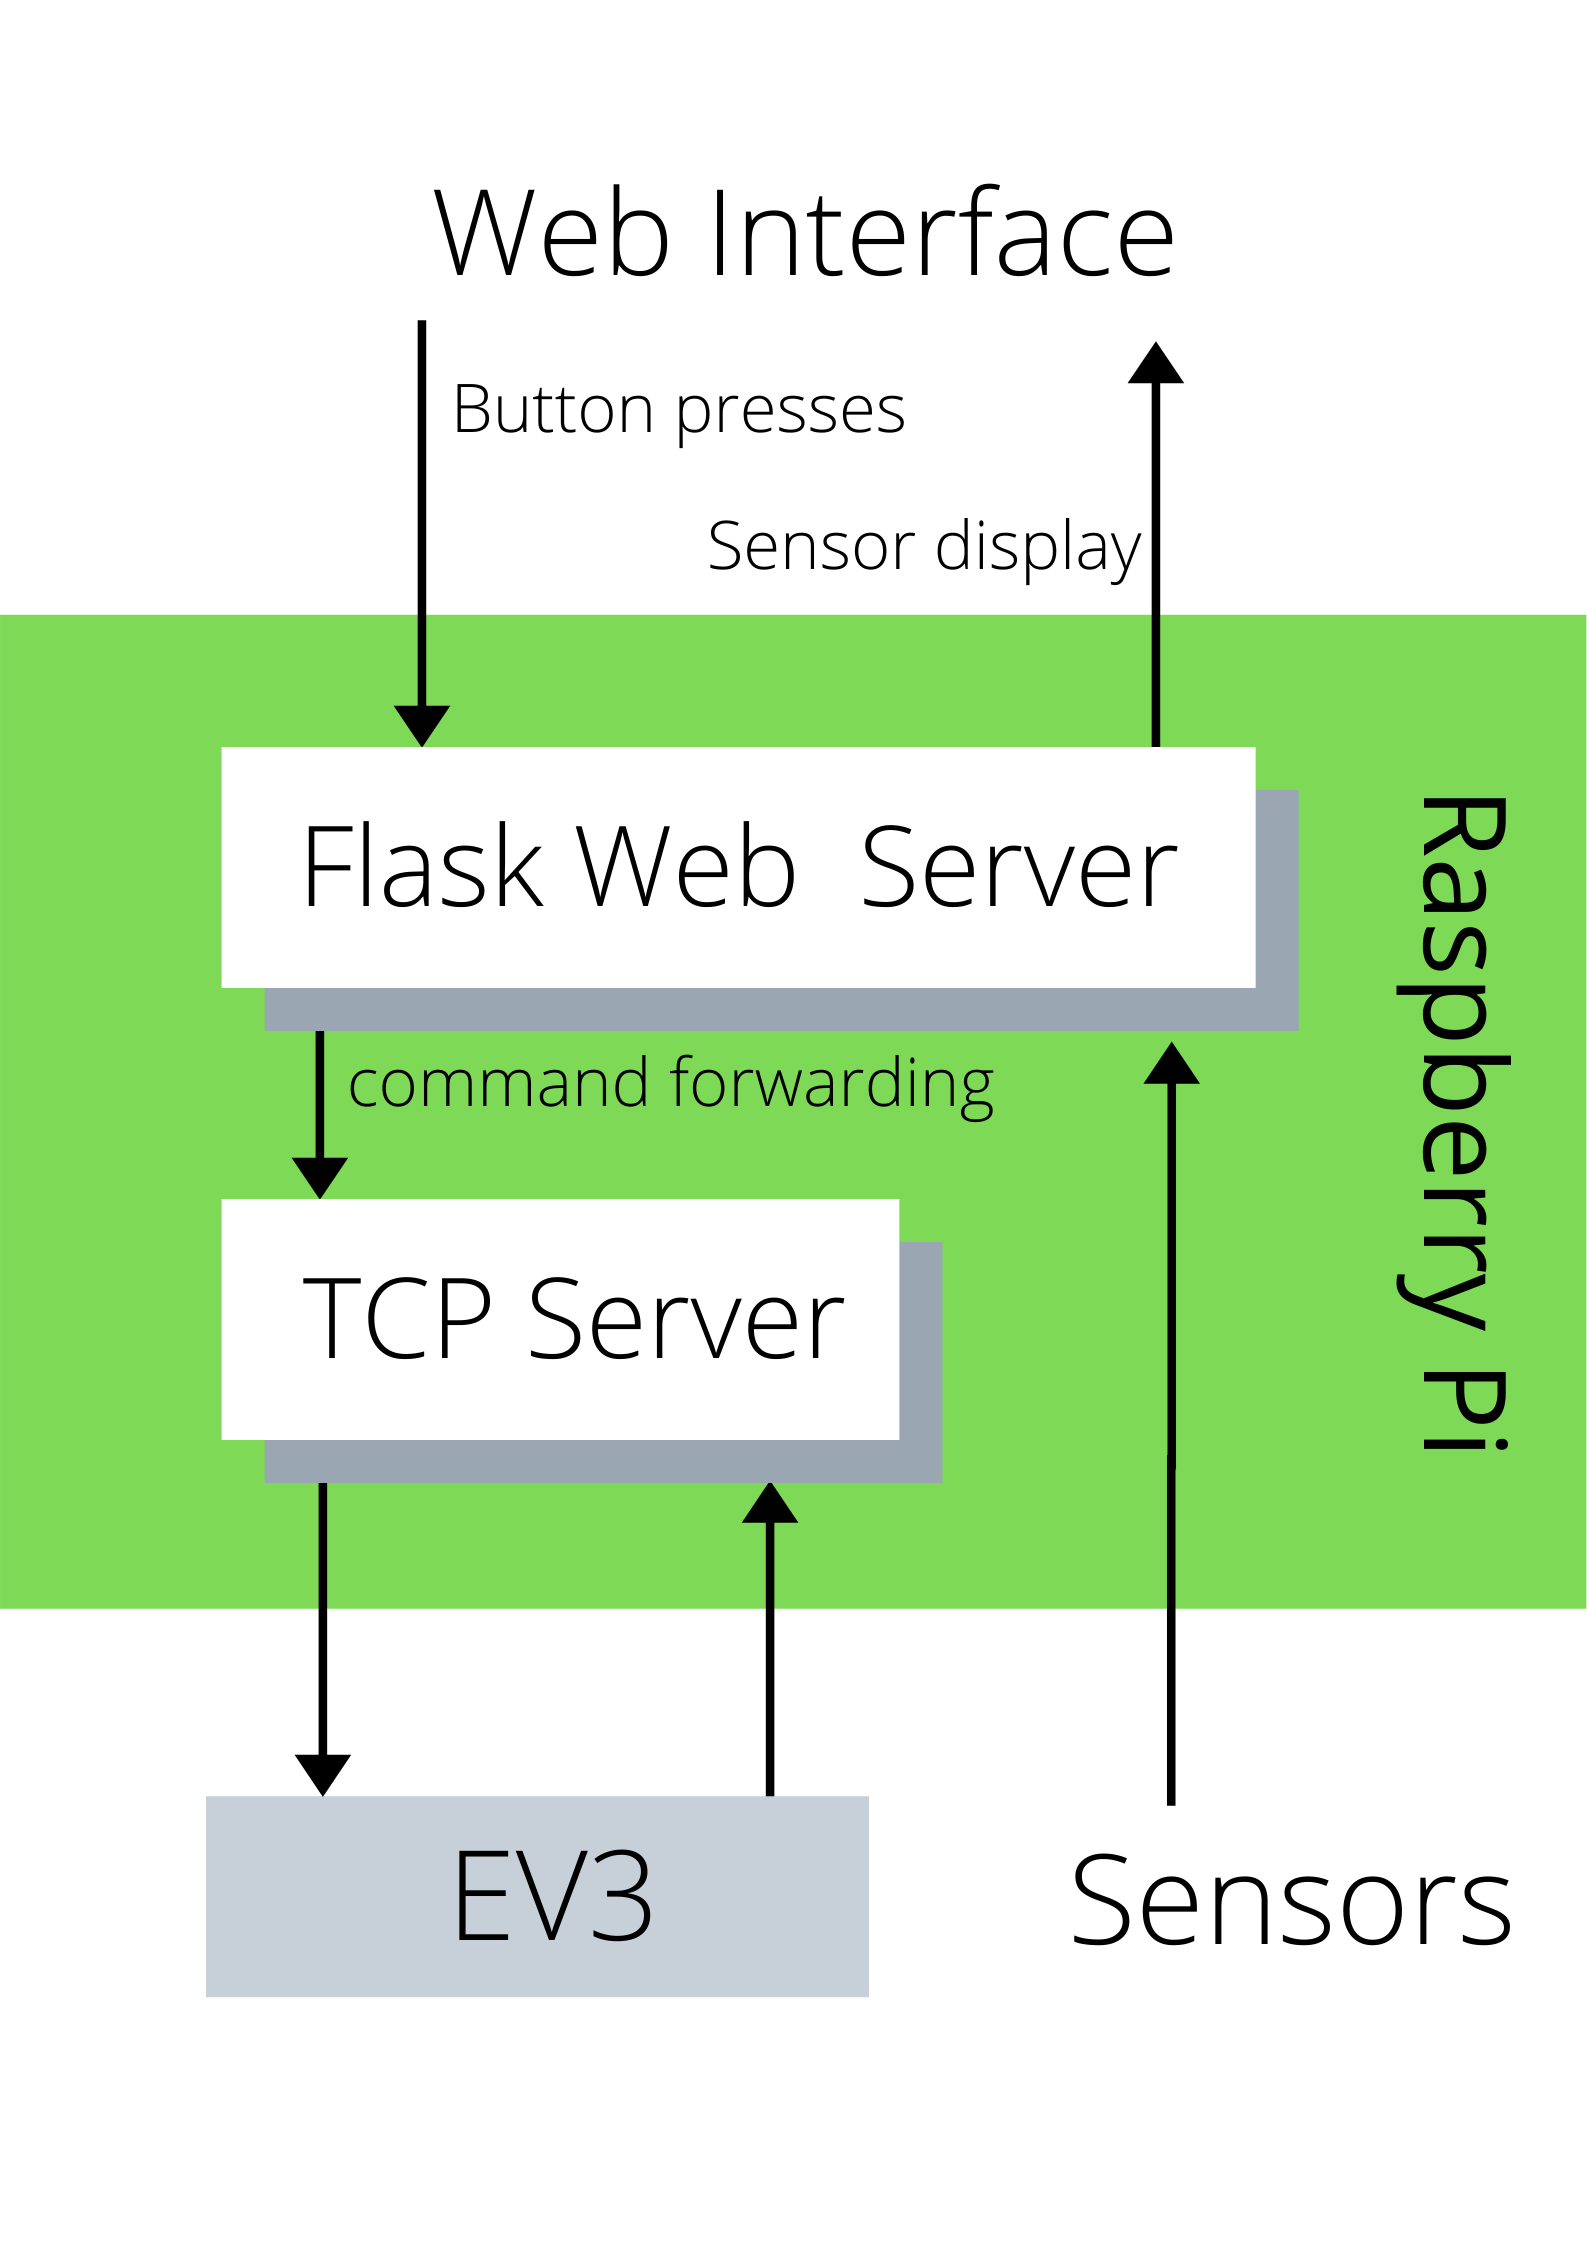
\includegraphics[height=190,keepaspectratio,width=1\linewidth]{figs/NetworkDiagram.png}    \caption{Flow of Data between the UI, Pi and EV3}
    \label{Network Diagram}
\end{figure}
\begin{figure}
    \centering
    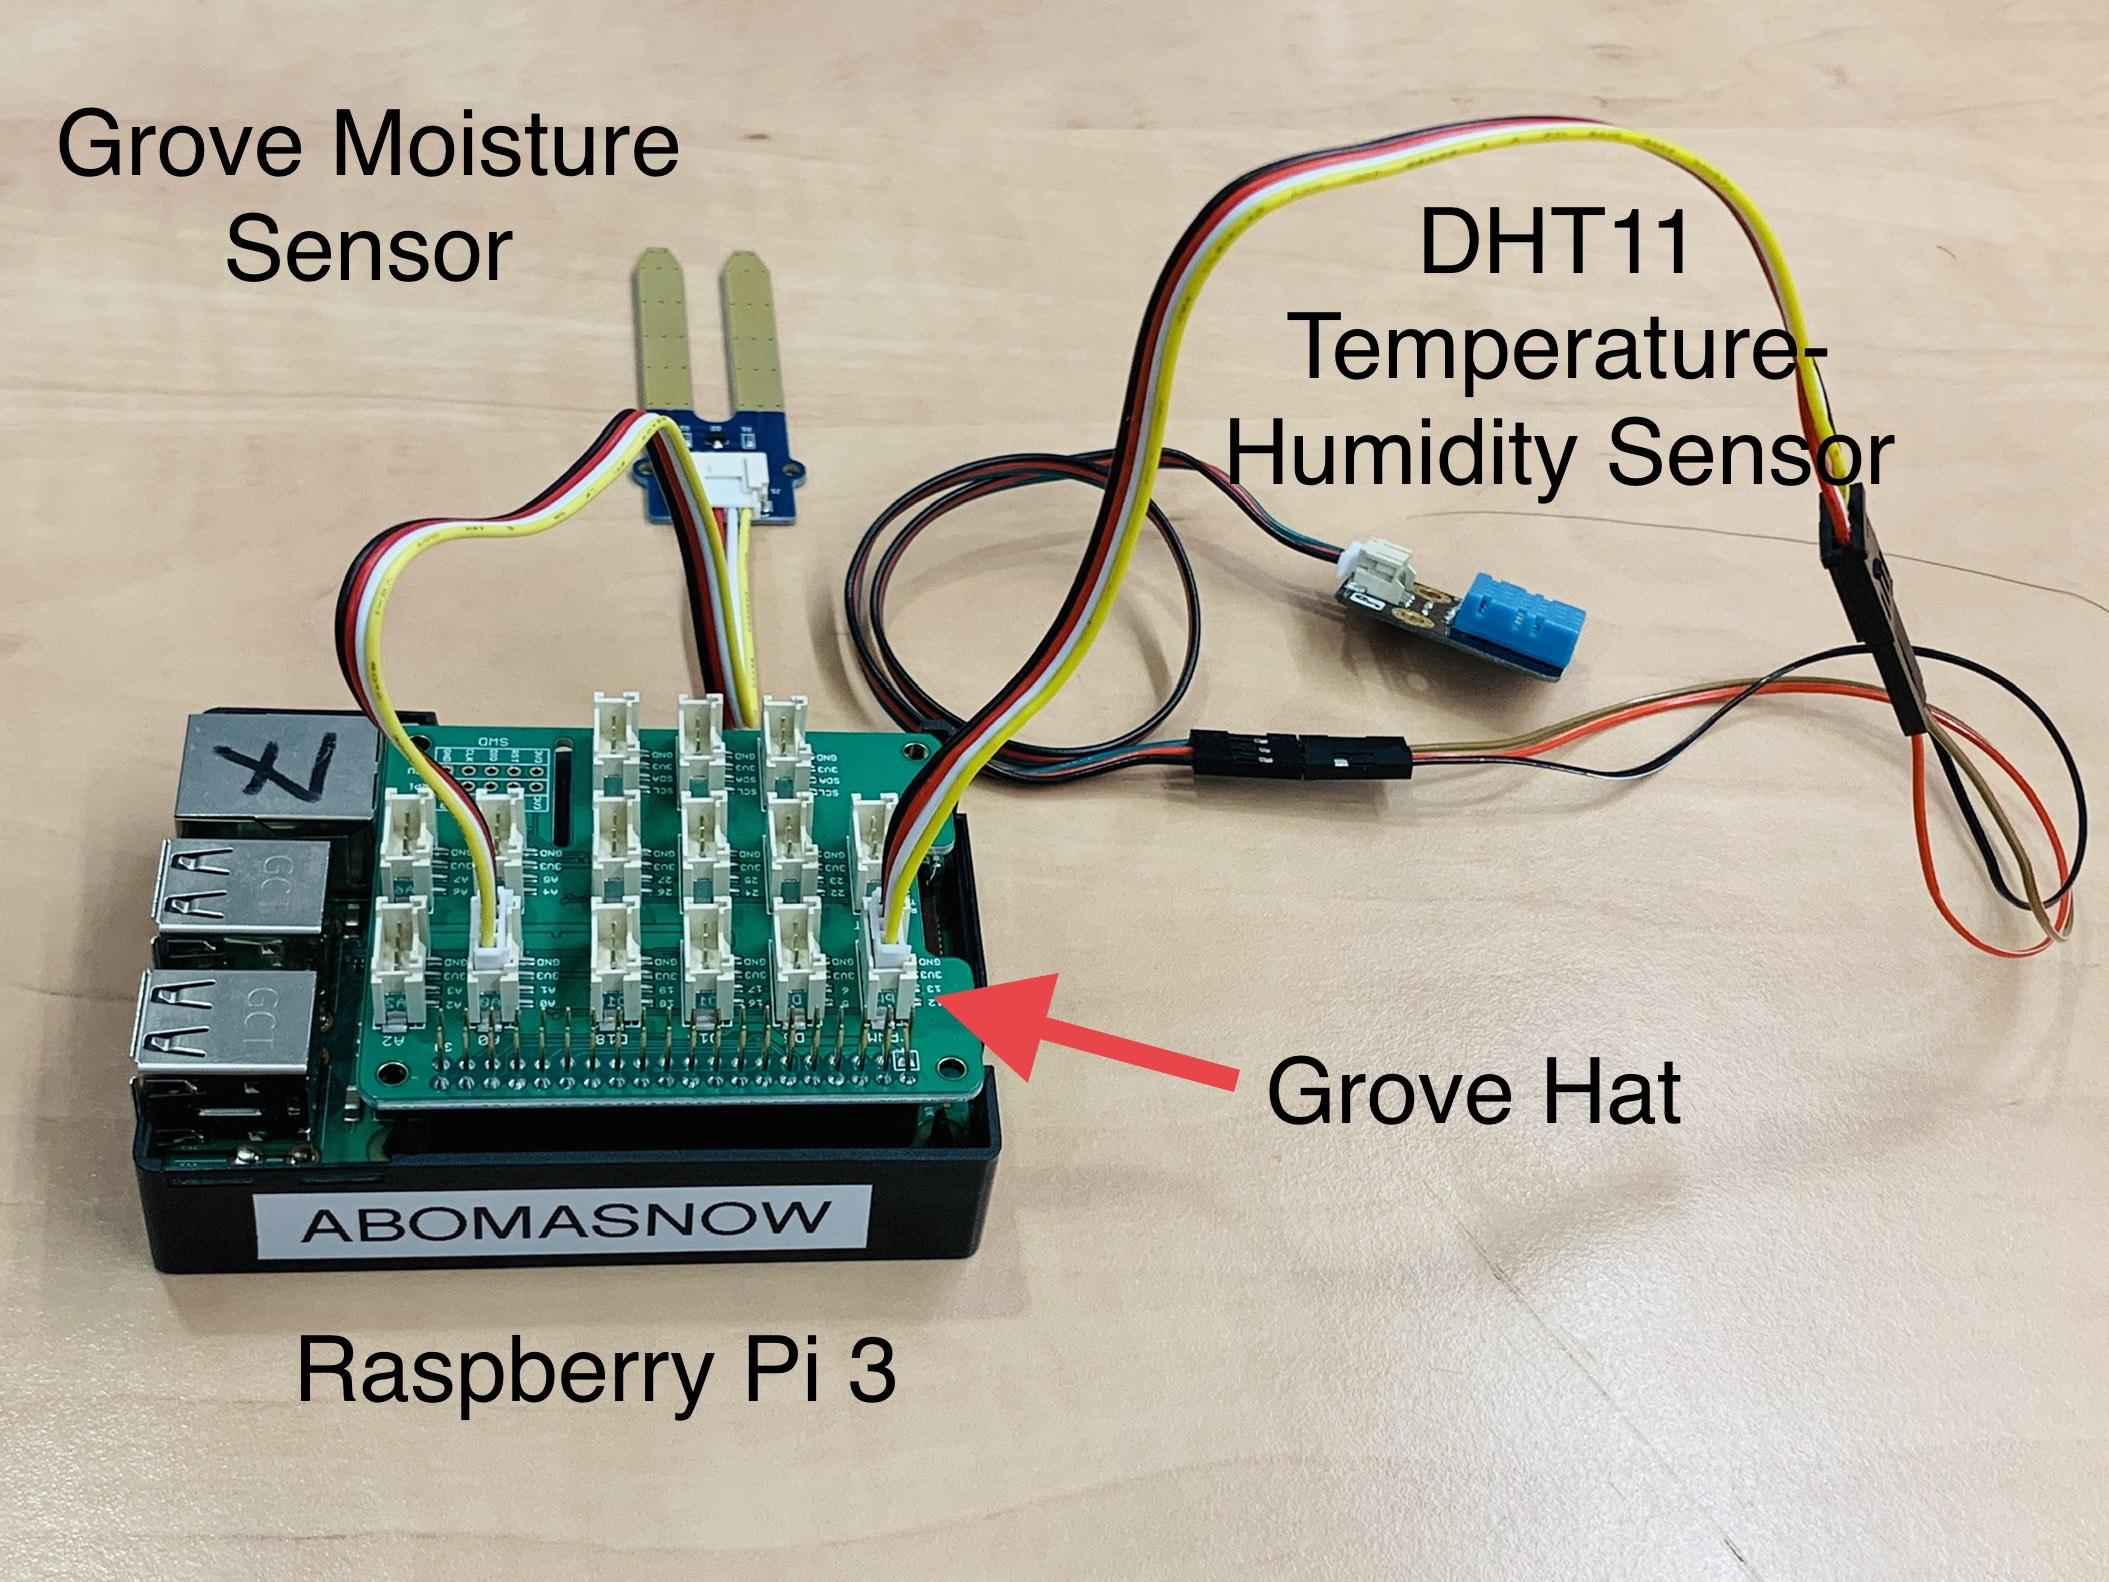
\includegraphics[height=150,keepaspectratio,width=1\linewidth]{figs/sensors_connection.jpeg}    \caption{Connection between sensors, Grove Hat and the Raspberry Pi}
    \label{Sensors Connection Diagram}
\end{figure}

The Grove Base Hat provides an interface for connecting sensors to the Raspberry Pi. We were able to connect the Grove moisture sensor to Grove Hat and after importing the necessary modules to fix the code error we could display the sensor data on the Raspberry Pi, after this it was trivial to add the temperature sensor.
An alternative to the Grove Base Hat is the Grove Pi+ for Raspberry Pi which is three times the price and offers data conversion features not necessary for our use case. 
We also created a button on the front-end that displays the current readings of the sensors to demonstrate communication between the sensors and the webapp. This information will be used in later stages by the front end team to display historical sensor information by the front end team.


\subsection{Web Application team}
We have used the Python web framework, Flask, to set up a web server on the Raspberry Pi. There are alternatives that we could have used, such as  Django, which is a full-stack framework, but for our project the lightweight and minimalist Flask framework provides all that we need for our web application. It was simple to set up a basic web app in just a few lines of code using Flask. It also does not use much of the Raspberry Pi’s resources, which is ideal since we also have a separate server running on the Pi for motor communication.

The usability prototype for the web app can be found at \href{https://www.figma.com/proto/2DwWDgggZoKzpLGs5jLPee/Sprout.ed?node-id=5\%3A3&scaling=contain}{this link}. Using a prototyping tool was more useful than using only paper and Google Slides to make wireframes - it allowed us to create an interactive design which we could give to users to test and receive feedback on its usability. We decided to use Figma to create the prototype. Alternative tools exist such as Just in mind, but Figma was recommended to Dima by a UI/UX professional for speed and ease of use. Even without previous experience using Figma we could easily create an interactive design as desired, and collaborate with multiple users editing the design simultaneously.

Building the wireframes and prototype of the web application allowed us to work out the best layout of the app. Both office workers and the office manager would want to use the application, but they would need access to different functionality. The normal office workers should be able to view the plants and their basic information, but they do not need a detailed breakdown of sensor information and should not be able to change settings or plant new plants. Therefore, we decided to have a Home page available to all the users with basic information, and an Admin Dashboard accessed by entering an admin password, with all the extra features for office managers.

Through the wireframes and prototyping we developed a layout for our web app which centred around a display of the planting bed with normal and admin views. This allowed for intuitive navigation of different features and meant that a navigation bar wasn't necessary, from our UX research we realised that this consistency between views leads to a smoother overall user experience.


During the development of the whole system it is necessary for us to be able to test different parts of the system, especially moving parts of the robot using motors and reading sensor data. For this, we created an Overrides page accessible from the Admin Dashboard, where we add in testing functionality (e.g. a button which causes the gantry to move forwards). This section of the web app is not necessary in the final implementation of the system for customers, but is essential while building the prototype.




\section{Evaluation}


The evaluation of the \textbf{mechanical system} was done using three standards for the moving bases: \textbf{balance}, \textbf{sturdiness}, and \textbf{weight distribution}.
\\
\vspace{-3mm}

\textbf{Balance} - tested by attaching the aluminium rod vertically on top of the base, trying to move the base back and forth along the rail and observing if the rod moves in a stable fashion (passed by all 3 iterations seen in figure 1). The base was also placed on the rail with the motor attached to see how it handles an offset to the centre of weight (only passed by 3rd iteration). \\
\textbf{Sturdiness} - tested by applying weight to the base directed downwards via the attached aluminium rod. All the iterations sustained pressure higher than they would encounter in standard operation.\\
\textbf{Weight distribution} - the position for center of mass was calculated to be equidistant from both of the parts in contact with the rail. This has been done for 1st and 2nd iterations, but will need to be recalculated for 3rd due to its different structure and adjust the printed parts accordingly. In the calculations, the weight distribution of the base itself was disregarded due to its trivial weight in comparison to the rod or the motor, and its relatively even distribution. 

To evaluate the prototype \textbf{web app} we first gave it to other members of the team who had not been working on it. We gathered feedback about the design, then implemented this, such as increasing font sizes for some text. We could also see if there were features that the rest of the team expected to be present that we had not included. For example, the ability to see more detailed information about a particular plant type from the Home page (accessible to all users), not just within the ‘Add a new plant’ feature (accessible only to admins).

We tested the updated prototype on a couple of users not involved in the project. This gave a better test of the usability of the application, since these testers were not aware of all the features present before using the app. This gave us more of an insight into how an actual user would use the application. These users commented that they liked the layout and appearance of the web application. By watching their interaction with the prototype, we were able to identify some changes to make to the user interface, such as making it clearer how to add a new plant.

Initially we faced a problem where the TCP server wasn't receiving messages from the clients. After doing a detailed code walk through, we figured that the Client code in the TcpCom library had a crucial line of code missing. Code walk throughs along with debug logs helped us spot errors that were more common and obvious. For testing whether the Raspberry Pi could connect to the EV3 and vice versa,  we used ping command of Linux. The ping command can tell if a computer can communicate with another computer over a network.

The evaluation of the system's \textbf{electrical} components was done through thorough testing under multiple different scenarios. For example, when testing the moisture sensor we tested if the readings displayed in the console changed under multiple environments, such as holding it with sweaty palms, putting it under the soil, and dipping it in a small flask of water. The readings of these measurements are shown in the table below. 

\begin{center}
 \begin{tabular}{||c c||} 
 \hline
 Situation & Reading \\ [0.5ex] 
 \hline
 In Dry Air & 0 \\ 
 \hline
 Sweaty Palms & 479 \\
 \hline
 Under Soil & 546 \\
 \hline
 Dipping under water & 1172 \\ [1ex]
 \hline
\end{tabular}
\end{center}

\section{Budget}\label{budget_account}
Please refer to the table below for an estimate of the budget for the overall system. 

\begin{figure}[b!]
    \centering
    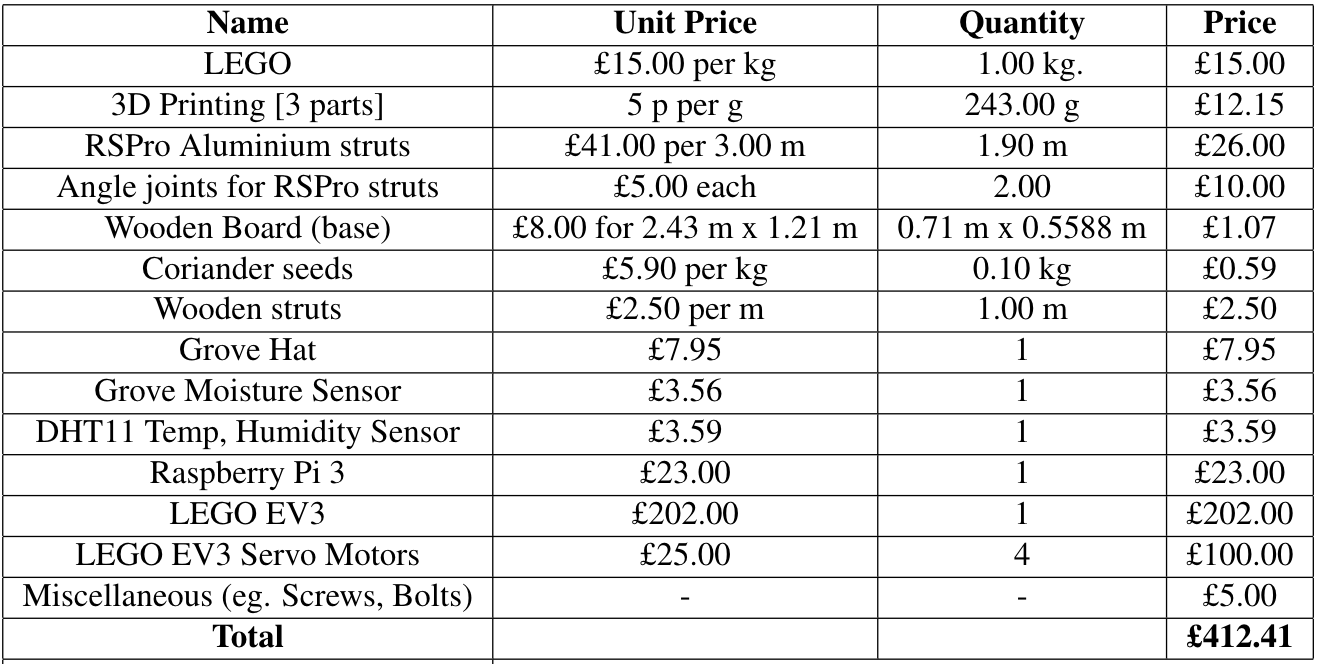
\includegraphics[width=375, angle = -90,keepaspectratio]{figs/budgettableNEW.png} 
    
\end{figure}

%% Include any references in a bibliography

%% \bibliography{example-refs} %%

\end{document} 

